\documentclass[tikz]{standalone}
\begin{document}

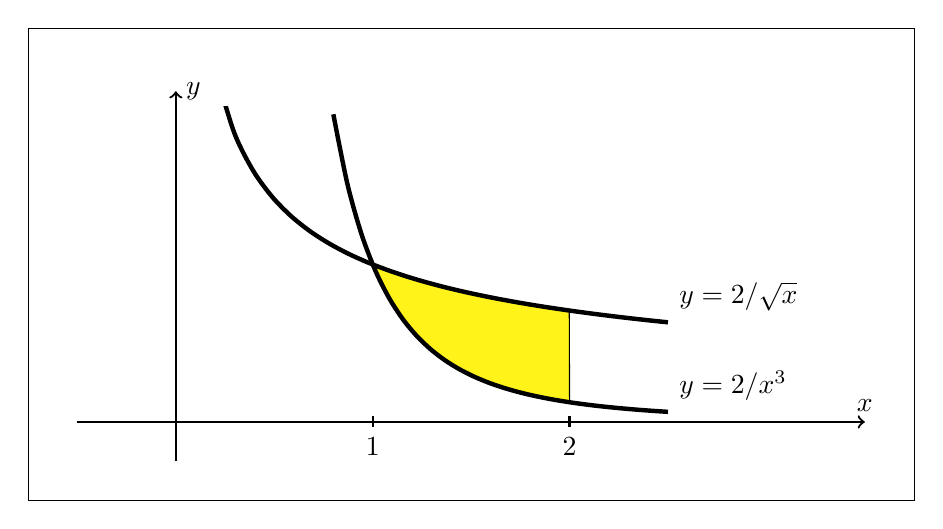
\begin{tikzpicture}[xscale=2.5]

  \draw[fill=white] (-0.75,-1) rectangle ++(4.5,6);

  % shade region
  \draw[fill=yellow!90] plot[smooth, samples=100, domain=1:2] ({\x},{2 / \x^0.5}) -- plot[smooth, samples=100, domain=2:1] ({\x},{2 / \x^3});

  %draw axes
  \draw[thick,->] (-0.5,0) -- (3.5,0) node[above] {$x$};
  \draw[thick,->] (0,-0.5) -- (0,4.2) node[right] {$y$};

  % draw curves
  \clip (0,-0.5) rectangle ++(3.4,4.5);
  \draw[ultra thick,domain=0.2:2.5,smooth,variable=\x,black] plot ({\x},{2 / \x^0.5}) node[above right] {$y=2/\sqrt{x}$};
  \draw[ultra thick,domain=0.8:2.5,smooth,variable=\x,black] plot ({\x},{2 / \x^3}) node[above right] {$y=2/x^3$};

  % tick marks
  \foreach \x in {1,2} 
    \draw [thick] (\x cm,2pt) -- (\x cm,-2pt) node[below] {$\x$};

\end{tikzpicture}
\end{document} 
